\documentclass[a4paper,twopage,ngerman,11pt]{scrreprt}


%
% Packages
%
\usepackage{pdfpages}
\usepackage{a4}
\usepackage[ngerman]{babel}
\usepackage[utf8]{inputenc}
%\usepackage[colorlinks=true,linkcolor=blue]{hyperref}st]{glossaries}
\usepackage{xcolor}
\usepackage[nonumberlist]{glossaries}
\usepackage{cite}
\usepackage{url}
\usepackage{graphicx}
\usepackage{bibgerm}
\usepackage{svn}
\usepackage{listings}
\usepackage{helvet}
\usepackage[bf]{caption}
\usepackage{color}

%
% Custom Commands
%
\newcommand{\HRule}{\rule{\linewidth}{0.5mm}}
%unused
\newcommand\etc{\textsl{etc}}
\newcommand\eg{\textsl{eg.}\ }
\newcommand\etal{\textsl{et al.}}
\newcommand\Quote[1]{\lq\textsl{#1}\rq}
\newcommand\fr[2]{{\textstyle\frac{#1}{#2}}}
\newcommand\miktex{\textsl{MikTeX}}
\newcommand\comp{\textsl{The Companion}}
\newcommand\nss{\textsl{Not so Short}}

%
% Document
%
\begin{document}

	% Titelseite
	%-----------------------------------------------------------
\begin{titlepage}
 
\begin{center}
 
 
% Upper part of the page

\includegraphics[width=0.15\textwidth]{./img/logo}\\[2cm]
 

 
\textsc{\Large Bachelor Arbeit}\\[0.5cm]
 
 
% Title
\HRule \\[0.4cm]
{ \huge \bfseries Handschrifterkennung mit Android}\\[0.4cm]
 
\HRule \\[1.5cm]
 
% Author and supervisor
\begin{minipage}{0.4\textwidth}
\begin{flushleft} \large
\emph{Autoren:}\\
Julian \textsc{Hanhart}\\
Dominik \textsc{Giger}
\end{flushleft}
\end{minipage}
\begin{minipage}{0.4\textwidth}
\begin{flushright} \large
\emph{Betreuer:} \\ 
Dipl. El.-Ing. ETH / BWI Alexander \textsc{Bosshard}\\
 
\end{flushright}
\end{minipage}
 
\vfill
 
% Bottom of the page
\textsc{Winterthur}\\
{\large \today}
 
\end{center}
 
\end{titlepage}
%-----------------------------------------------------------
	

	% Abstract / Management Summary (ev. Abstract on Title-Page)
	%\selectlanguage{ngerman}

\begin{abstract}
\chapter*{Zusammenfassung}
\thispagestyle{empty}
\selectlanguage{ngerman}

\begin{abstract}
\chapter*{Zusammenfassung}
\thispagestyle{empty}
\selectlanguage{ngerman}

\begin{abstract}
\chapter*{Zusammenfassung}
\thispagestyle{empty}
\input{../abstract/abstract.txt}
\end{abstract}

\begin{otherlanguage}{english}
\begin{abstract}
\chapter*{Abstract}
\thispagestyle{empty}
\input{../abstract/abstract_en.txt}
\end{abstract}
\end{otherlanguage}
\end{abstract}

\begin{otherlanguage}{english}
\begin{abstract}
\chapter*{Abstract}
\thispagestyle{empty}
\input{../abstract/abstract_en.txt}
\end{abstract}
\end{otherlanguage}
\end{abstract}

\begin{otherlanguage}{english}
\begin{abstract}
\chapter*{Abstract}
\thispagestyle{empty}
\input{../abstract/abstract_en.txt}
\end{abstract}
\end{otherlanguage}
	\begin{abstract}
	Dies ist das Abstract
	\end{abstract}
	

	% BA Erklärung
	
\includepdf[pagecommand={\thispagestyle{plain}},scale=1.0]{inc/Erklaerung_BA.pdf}
		

	% Römische Seitenzahlen
	\newpage
	\renewcommand{\thepage}{\Roman{page}}
	\setcounter{page}{1}
	
	% Content
	\tableofcontents

	% Verzeichnisse
	% Abbildungen
	\listoffigures
	% Tabellen
	\listoftables
	% Listings
	\definecolor{listingbg}{HTML}{99CCCC}
	\lstset{language=Java}
	\lstset{backgroundcolor=\color{listingbg}, frame=single,framerule=0pt,firstnumber=auto, numbers=left, numberstyle=\tiny, stepnumber=1, numbersep=8pt, captionpos=b}
	\lstlistoflistings
	
	% Begin Inhalt
	% Seitenzahl auf Arabisch wechseln
	\newpage
	\renewcommand{\thepage}{\arabic{page}}
	\setcounter{page}{1}
	

	\part{Einleitung}
		\chapter{Aufgabenstellung}
		
		\chapter{Vorgehensweise}
		
		\chapter{Aufbau Report}

	\part{Theoretischer Hintergrund}
		\chapter{Mikro Gesten}
		\section{Definition}
		\section{Typen}
		\section{Abbildung von Zeichen}

		\chapter{Graph}
		\section{Funktionsweise}
		\section{Erkennung von Zeichen}

	\part{Lösung}
		% Verschiedene Ansätze beschreiben
		%\chapter{Prototyp}
		\chapter{Mikrogesten-Erkennung}

Nach der Sichtung der vorgegangen Projektarbeit haben wir uns entschieden, dass zwei Ansätze zur Erkennung der einzelnen Mikrogesten aus der Eingabe-Menge an Punkten im Prototyp ausprobiert und evaluiert werden sollten. Zum einen sollte die in der Projektarbeit favorisierte Erkennung durch die Änderung der Krümmung zwischen den einzelnen Punkten getestet werden, zum Anderen ein Ansatz ausprobiert werden, der auf einer auf dem vorausgehenden Punkt basierenden Voraussage des jeweils als nächstes folgenden Punktes aufbaut.

Der Krümmungs-Ansatz wurde in der vorgängigen Projektarbeit neben einem auf der Änderung der Winkel zwischen Punkten basierenden Ansatz zur Mikrogesten-Erkennung evaluiert und am Ende von den Autoren der Arbeit favorisiert. Dadurch war klar, dass wir diese Art der Erkennung ebenfalls für diese Arbeit evaluieren sollten.

Neben einer Erkennung durch die Krümmungs- und die Winkel-Änderung zwischen Punkten sollte unserer Meinung nach auch eine Erkennung durch die Voraussage von folgenden Punkten möglich sein und wurde daher von uns ebenfalls implementiert und evaluiert.

Diese Ansätze bewährten sich für die Variante A der Mikrogesten, jedoch gab es gewisse Schwierigkeiten, die Mikrogesten der Variante B zu erkennen. Um Spezialfälle wie z.B. einen Kreis zu erkennen, haben wir zusätzliche Algorithmen entwickelt, die nur eine sehr spezialisierte Aufgabe erfüllen. So gibt es zum Beispiel einen Algorithmus, der nur Linien erkennt und einen, der nur Halbkreise erkennt.

\section{Bewertungs-Kriterien}

\begin{table}[h!]
  \begin{center}
    \begin{tabular}{ m{2.2cm} |  p{10cm} }
    \emph{Kriterium} & Erkennungszuverlässigkeit  \\ \hline
    \emph{Beschreibung} & Um eine verlässliche Erkennung der Mikrogesten zu ermöglichen, muss ein Ansatz natürlich gewährleisten, dass er die Auftrennung der Mikrogesten zuverlässig vornimmt. \\ \hline
    \emph{Priorität} & Primär  \\
    \end{tabular}
  \end{center}
  \caption{Kriterium Erkennungszuverl\"{a}ssigkeit}
  \label{kriterium_erkennungszuverlaessigkeit}
\end{table}

\begin{table}[h!]
  \begin{center}
    \begin{tabular}{ m{2.2cm} |  p{10cm} }
    \emph{Kriterium} & Toleranz  \\ \hline
    \emph{Beschreibung} &

 Obwohl die Erkennung natürlich zuverlässig sein sollte, muss aber auch eine gewisse Toleranz für nicht ideale Eingaben gewährt werden. Da die Handschriften-Erkennung auf Menschen und einen Einsatz im mobilen Umfeld ausgerichtet werden soll, sind suboptimale Eingabefolgen durchaus zu erwarten und die Erkennung der Mikrogesten sollte daher einigermassen tolerant auf solche reagieren. Dies stellt offensichtlich ein Zielkonflikt zum Zuverlässigkeits-Kriterium dar und es muss daher ein guter Mittelweg zwischen diesen beiden Kriterien gefunden werden. 
\\ \hline
    \emph{Priorität} & Primär  \\
    \end{tabular}
  \end{center}
  \caption{Kriterium Toleranz}
  \label{kriterium_toleranz}
\end{table}

\begin{table}[h!]
  \begin{center}
    \begin{tabular}{ m{2.2cm} |  p{10cm} }
    \emph{Kriterium} & Performanz  \\ \hline
    \emph{Beschreibung} &

 Auf einem mobilen System ist der schonende Umgang mit den Systemressourcen besonders wichtig und das Verfahren zur Erkennung der Mikrogesten sollte daher möglichst wenig Rechenleistung brauchen. Da es allerdings nur jeweils nach Benutzereingaben durchgeführt werden muss und eine Ausführung im Hintergrund möglich sein sollte, könnten gewisse Abstriche in diesem Bereich unter Umständen in Kauf genommen werden.
\\ \hline
    \emph{Priorität} & Sekundär  \\
    \end{tabular}
  \end{center}
  \caption{Kriterium Performanz}
  \label{kriterium_performanz}
\end{table}

%================================================
\section{Verfahren zur Auftrennung des Pfades}
\subsection{Ansatz: Punkte-Voraussage}
%TODO Ev. diesen Satz etwas einfacher formulieren
Grundlage des auf Voraussage des jeweils nächsten Punktes basierenden Ansatzes sollte die Annahme sein, dass man den als nächstes auf einen Punkt einer gleichmässig gekrümmten Kurve folgenden Punkt durch das Spiegeln des jeweils dem Ausgangspunkt vorangehenden Punktes an der Achse des Ausgangspunktes vorherbestimmen können müsste. Weicht der tatsächlich eingegebene Folgepunkt zu sehr vom vorausgesagten Folgepunkt ab, sollte nun angenommen werden, dass dieser Punkt nicht mehr zur aktuellen Mikrogeste gehören und als Ausgangspunkt einer neuen Mikrogeste genommen werden soll.


\subsubsection{Bewertung}
Die grundsätzliche Trennung der einzelnen Mikrogesten durch das auf Voraussagen basierende Verfahren wurde von uns als durchaus zufriedenstellend bewertet. Das Verfahren ermöglicht die Auftrennung der Eingabepunkte in verschiedene Mikrogesten. Allerdings erkennt das Verfahren unserer Meinung nach leider zu viele einzelne Mikrogesten und ist zu wenig tolerant gegenüber kleineren Abweichungen. Schon kleinere Änderungen in der Linienführung führen dabei zu einer Auftrennung von ansonsten durchaus zusammenhängenden Gesten.

Auch weist das Verfahren Probleme mit ungleichen Punktedichten auf einem Pfad auf. Dies tritt vor allem auf, wenn die Eingabegeschwindigkeit variiert, etwa wenn nach einer Richtungsänderung oder am Anfang einer Geste die Eingabe beschleunigt wird und die späteren Eingabepunkte weiter auseinander liegen als die ersten. Gerade bei unregelmässigen Beschleunigungen kommt es somit häufig vor, dass die ersten Eingabepunkte relativ nahe beieinander liegen, der Abstand zu späteren Punkten dann aber recht gross wird. Die vorausgesagten Punkte mögen dann zwar durchaus auf dem Pfad der Geste liegen, die Eingabepunkte folgend dann allerdings erst in grösserem Abstand. Diesem Verhalten könnte möglicherweise mit Anpassungen an der Berechnung der vorausgesagten Punkte begegnet werden. Man könnte etwa anstatt eines konkreten Punktes eine Richtung voraussagen. Auch ein normierter Abstand zwischen den Eingabepunkten, wie ihn das Spline-Glättungsverfahren erzeugt, welches als mögliche Optimierung in \ref{sec:Glaettung} besprochen wird. Eine Glättung der Eingangspunkte sollte auch die Toleranz des voraussagenden Ansatzes verbessern können.

Weiter haben wir mit diesem Verfahren Probleme mit zu nahe beieinander liegenden Eingabepunkten festgestellt. Ist die Distanz von einem Punkt zum nächsten kleiner als die Länge des Toleranz-Wertes, fällt der Punkt in jedem Fall innerhalb der Toleranz und es kann keine fundierte Aussage über mehr darüber gemacht werden, ob der Punkt zur selben Mikrogeste gehören soll oder nicht. Daher werden nur Punkte, deren Abstand zum Ausgangspunkt kleiner als die zweifache Länge des Toleranz-Wertes sind, beachtet. Andere Punkte werden als zur aktuellen Mikrogeste gehörig angenommen und zum neuen Ausgangspunkt. Dies führt wiederum zu Problemen mit sehr engen Kurven, wie sie etwa bei Richtungswechseln und sehr eng-winkligen Spitzen, da diese eng beieinander liegende Eingabepunkte erzeugen, deren Abstand häufig unterhalb die Toleranzgrenze fällt. Somit wird häufig noch der erste Punkt nach einer solchen Spitze zur vorherigen Mikrogeste zugeordnet.

Diesen beiden Probleme, welche beide das als substantiell gewertete Bewertungskriterium der Toleranz beeinträchtigen, steht steht nur eine gute Performanz durch die relativ simplen Berechnungen, die das Voraussage-Verfahren benötigt, gegenüber. Da das Toleranz-Kriterium von uns aber als signifikant wichtiger eingestuft wurde und vom Krümmungs-Verfahren weit besser erfüllt wird, mussten wir uns am Ende für das auf Krümmungs-Änderungen basierende Verfahren festlegen.

%================================================

\subsection{Ansatz: Krümmungs-Änderung}
Das Krümmungsverfahren basiert auf dem Verfahren, das in \cite{zeichenerkennung_pa} vorgeschlagen wird: Die Punkte eines Pfades werden mit Vektoren verbunden. Zwischen jedem Vektor und seinem Nachfolger wird nun das Kreuzprodukt (siehe Abbildung \ref{kreuzprodukt}) gebildet. Das Vorzeichen des Resultats gibt nun die Drehrichtung der Kurve an. Die Änderung der Drehrichtung ist bereits eine wichtige Information um den Pfad in Mikrogesten zu unterteilen.
Als zweite Information erhält man den Winkel zwischen den Vektoren. Nun kann man den Pfad an den Stellen trennen, wo der Winkelunterschied zu den vorherigen Vektoren eine gewisse Toleranz überschreitet. Dies ist vor allem nützlich um zwischen einer starken und einer schwachen Krümmung zu unterscheiden.

\begin{figure}[h!]
  \centering
    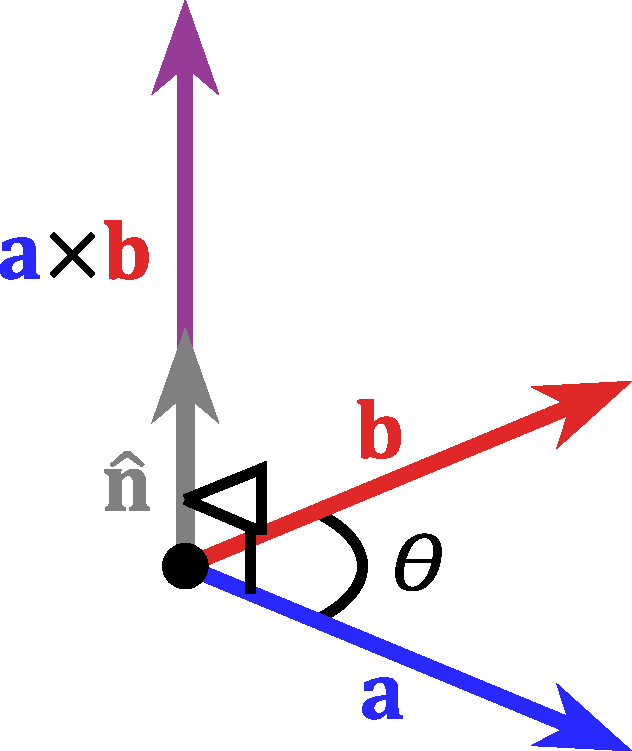
\includegraphics[width=0.3\textwidth]{./img/crossproduct.pdf}
  \caption{Kreuzprodukt zweier Vektoren}
  \label{kreuzprodukt}
\end{figure}

\subsubsection{Verfahren}
Das Vorgehen bei diesem Algorithmus ist sehr simpel: Es wird laufend die Krümmung zwischen dem aktuellen Punkt und seinen Nachbarn berechnet. Sobald die Krümmung einen gewissen Toleranzwert überschreitet wird der Pfad in zwei Mikrogesten aufgetrennt. Der genaue Ablauf ist in Abbildung \ref{curvatureflowchart} ersichtlich.

\begin{figure}[h!]
  \centering
    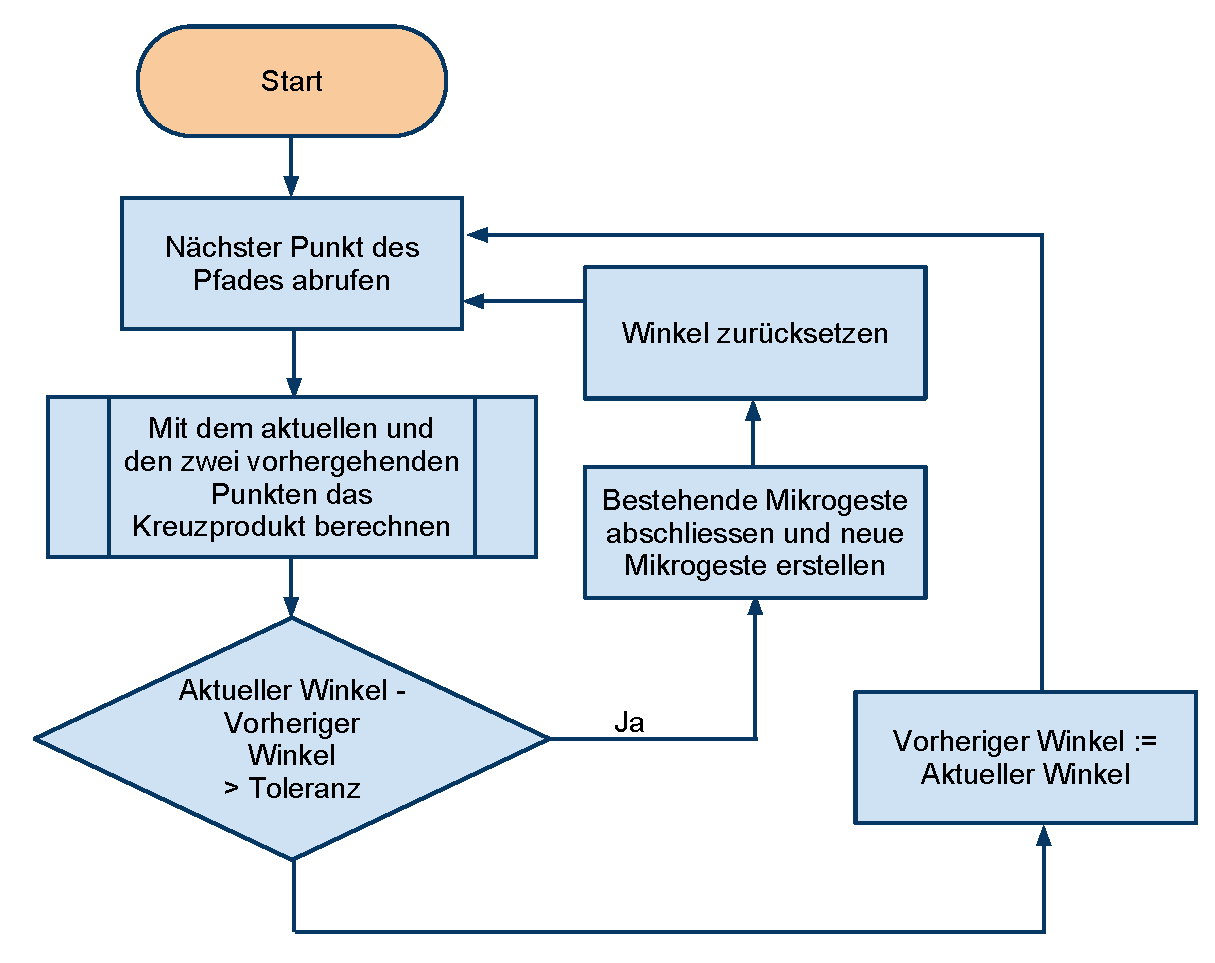
\includegraphics[width=\textwidth]{./img/CurvatureFlowchart.pdf}
  \caption{Ablauf des Krümmungs-Algorithmus}
  \label{curvatureflowchart}
\end{figure}

\subsubsection{Bewertung}
Das Verfahren is vor allem gut geeignet um Änderungen in der Drehrichtung zu erkennen (Nützlich z.B. bei dem Buchstaben 'S') und zwischen starken und schwachen Krümmungen zu unterscheiden. Es hat allerdings die gleichen Probleme wie die Punkte-Voraussage: Die Eingangspunkte müssen gut normiert sein um gleichmässige Erkennung zu garantieren. Dieses Problem kann jedoch mit einer Vorbearbeitung des Pfades gelöst werden.

%================================================

\subsection{Ansatz: Drehrichtungs-Erkennung}
Dieser Ansatz ist eine Abwandlung des Krümmungs-Verfahrens und so abgeändert, dass Drehrichtungsänderungen möglichst genau erkannt werden können. Der Hintergedanke dabei ist dass man bei Mikrogesten nur noch zwischen Kurven unterscheidet, die in eine andere Richtung drehen, aber nicht mehr die Stärke der Krümmung berücksichtigt.

\subsubsection{Verfahren}
Das Verfahren funktioniert prinzipiell gleich wie das Krümmungs-Verfahren: Es wird immer für zwei benachbarte Vektoren das Vektorprodukt berechnet. Der errechnete Wert wird immer zu einem Akkumulator addiert und mit dem Punkt abgespeichert. Nach dem der komplette Pfad so durchgerechnet wurde, erhält man eine Akkumulator-Kurve. In Abbildung \ref{drehrichtungsBeispiel} ist eine Beispiel-Eingabe gezeigt und in Abbildung \ref{akkumulatorDiagramm} der dazu berechnete Akkumulator-Verlauf. Wie man sieht stellen die Maxima und Minima der Kurve die Richtungswechsel in der Eingabe dar. Die Trennungspunkte können also durch ein einfaches berechnen aller lokalen Maxima und Minima bestimmt werden.

\begin{figure}[h!]
  \centering
    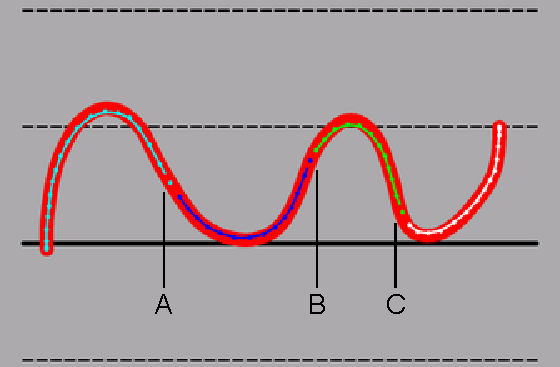
\includegraphics[width=0.67\textwidth]{./img/akkumulator_beispiel.pdf}
  \caption{Beispiel-Eingabe: rot, Erkannte Trennungen: Farbig.}
  \label{drehrichtungBeispiel}
\end{figure}

\begin{figure}[h!]
  \centering
    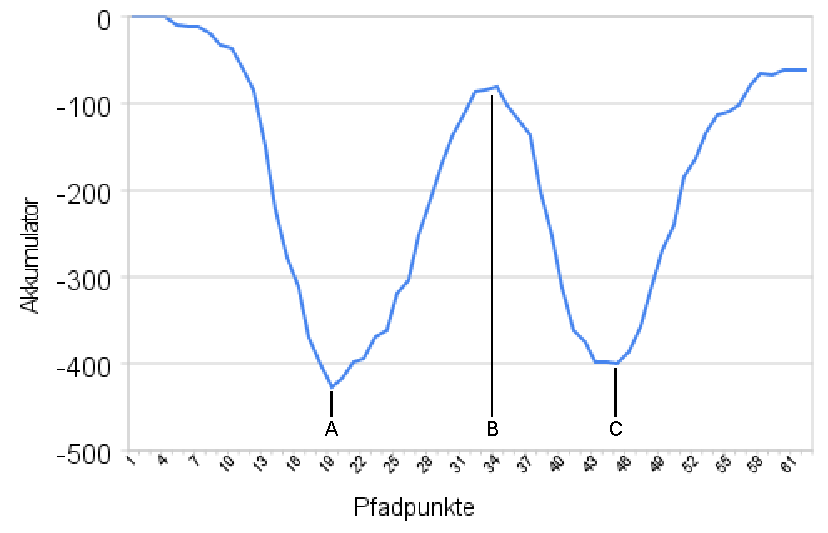
\includegraphics[width=1.0\textwidth]{./img/akkumulator_diagramm.pdf}
  \caption{Akkumulator für die Eingabe von Abbildung \ref{drehrichtungBeispiel}.}
  \label{akkumulatorDiagramm}
\end{figure}

\subsubsection{Bewertung}
Dieser spezialisierte Algorithmus funktioniert sehr gut, wenn der Pfad tatsächlich nur aus Kurven besteht. Deshalb ist es nötig, dass mit einem anderen Algorithmus alle Geraden aus dem Pfad entfernt wurden (Zum Beispiel dem Krümmungsalgorithmus).

%================================================

\subsection{Ansatz: Winkel-Änderung}

Dieses Verfahren funktioniert prinzipiell wie das Krümmungs-Verfahren. Es ist jedoch vereinfacht und berücksichtigt nur noch den Winkel zwischen zwei benachbarten Vektoren.

\subsubsection{Verfahren}
Es wird der Winkel zwischen den Vektoren berechnet und mit der Toleranz verglichen. Bei einem genügend spitzigen Winkel wird der Pfad aufgetrennt. Abbildung \ref{kanten_trennung} zeigt ein Beispiel einer Trennung.

\lstinputlisting [caption={Pseudocode-Algorithmus um scharfe Kanten im Pfad zu erkennen},label=edgesalgorithmus]{code/edges.pseudo}

\begin{figure}[h!]
  \centering
    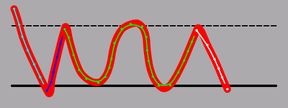
\includegraphics[scale=0.75]{./img/edges_beispiel.png}
  \caption{Beispiel einer Trennung: Jede farbige Linie ist eine erkannte Mikrogeste.}
  \label{kanten_trennung}
\end{figure}

\subsubsection{Bewertung}
Dieses Verfahren ist sehr einfach gehalten und darauf spezialisiert, Spitzkehren im Pfad zu erkennen. Der grosse Nutzen dieses Verfahren ist aber, dass der Pfad nicht normiert werden muss. Die anderen Verfahren erkennen zwar Spitzkehren auch, brauchen aber einen normierten, am besten geglätteten, Pfad. Die Glättung schwächt aber Spitzkehren ab und macht sie ev. sogar unkenntlich.  

%================================================

\subsection{Ansatz: Kreis-Erkennung}
Mit diesem Ansatz sollen alle geschlossenen Kreise auf dem Pfad erkannt werden. Alle restlichen Punkte werden nicht berücksichtigt und müssen mit einem anderen Verfahren aufgetrennt werden.

\subsubsection{Verfahren}
Mit jedem Punkt auf dem Pfad werden alle nachfolgenden Punkte verglichen: Wenn die zwei Punkte sehr nahe beieinander liegen bildet der Pfad zwischen den Punkten ein Kreis.

\lstinputlisting [caption={Pseudocode-Algorithmus um Kreise auf einem Pfad zu erkennen},label=kreisalgorithmus]{code/circle.pseudo}

\begin{figure}[h!]
  \centering
    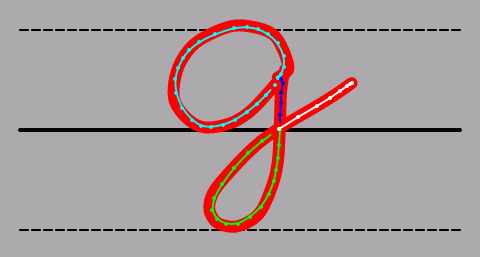
\includegraphics[scale=0.5]{./img/circle_beispiel.png}
  \caption{Beispiel einer Kreiserkennung: Farbige Linien stellen Mikrogesten dar.}
  \label{kreis_trennung}
\end{figure}

\subsubsection{Bewertung}
Die Kreiserkennung ist natürlich nur sinnvoll, wenn man eine entsprechende Mikrogeste "Kreis" hat. Allerdings gibt es auch beim Algorithmus noch Verbesserungsbedarf: Bei einem Spezialfall, nämlich ein Pfad der eine '8' bildet, wird der gesamte Pfad als ein Kreis erkannt und nicht als zwei Kreise. 


%================================================
\subsection{Fazit}
Es hat sich gezeigt, dass es nicht sinnvoll ist, sich auf ein einzelnes Verfahren zu stützen. Jedes Verfahren hat seine Schwächen, welche von einem anderen Verfahren abgedeckt werden können. Es ist am besten, den Pfad schrittweise zu unterteilen und bei jedem Schritt die Mikrogesten-Erkennung zu starten. Mit jedem weiteren Schritt werden dann nur noch Pfadteile berücksichtigt, welchen noch keine Mikrogeste zugewiesen ist.

%================================================

\section{Erkennung der Mikrogesten-Art}
Die Erkennung der Mikrogeste kann je nach Form der Mikrogeste unterschiedlich aufwändig sein. Deshalb haben wir für beide Mikrogesten-Varianten eigene Erkennungsalgorithmen erstellt:

\subsection{Variante A}
%% TODO sollte noch etwas erweitert werden
Für diese Variante ist die Unterscheidung von Line, schwacher Krümmung und starker Krümmung nötig. Die Erkennung ist deshalb recht einfach: Die Stärke der Krümmung unterscheidet alle Mikrogesten voneinander.

\subsubsection{Kreisradius berechnen}
Ein einfaches Verfahren zur Kategorisierung ist folgendes: Es wird mit einem Kreis die Punktemenge der Mikrogeste angenähert. Mit dem Radius dieses Kreises kann dann die Art der Geste bestimmt werden:
\begin{itemize}
\item \emph{Kleine Radien:} Starke Krümmung
\item \emph{Unendlich grosse Radien:} Linie
\item \emph{Rest:} Schwache Krümmung
\end{itemize}

\subsection{Variante B}
%% TODO MIt einem Flussdiagramm beschreiben
Für diese Variante läuft die Erkennung in mehreren Schritten ab:
\begin{enumerate}
\item Es werden mit dem Kreis-Algorithmus alle Kreise bestimmt.
\item Danach werden von den restlichen Mikrogesten die Geraden bestimmt. Dies wird sichergestellt, indem vom ersten zum letzten Punkt eine Linie gezogen wird. Wenn kein Punkt der Mikrogeste zu stark von der Linie abweicht, ist die Mikrogeste eine Gerade.
\item Alle übrigen Mikrogesten sind nun entsprechend automatisch Kurven.
\end{enumerate}

Diese Schrittweise Erkennung ist notwendig, da nach jedem Erkennungsschritt die übrigen Pfadteile in weitere Mikrogesten aufgeteilt werden.

%================================================

\section{Erkennung der Ausrichtung einer Mikrogeste}
Für jede Mikrogeste muss auch die Richtung bestimmt werden. Im Endeffekt gibt es nur vier verschiedene Richtungen, wie im theoretischen Teil beschrieben. 
\subsubsection{Richtung der Gerade}
Die Richtungsbestimmung einer Geraden ist sehr simpel, da die Steigung der Geraden direkt die Richtung darstellt.
\subsubsection{Richtung der Krümmungen}
Hier wird eine Gerade an die Krümmung approximiert und so die Richtung bestimmt.
\subsubsection{Richtung der Halbkreise}
%% TODO mit einem Diagramm darstellen
Für die Halbkreise ist die Richtungs-Bestimmung etwas schwieriger. Hier wird bestimmt, in welche Richtung die Öffnung zeigt.
Dazu wird zuerst bestimmt, ob die Öffnung oben/unten oder links/rechts ist. Wenn beide Endpunkte in etwa gleiche y-Werte haben ist die Öffnung oben/unten, wenn sie etwa gleiche x-Werte haben ist die Öffnung links-rechts.
Um zu bestimmen ob die Öffnung nun oben oder unten ist, muss nur die Anzahl der Punkte bestimmt werden, deren y-Werte unter denen der beiden Endpunkte liegt. Liegen die meisten Punkte darunter, ist die Öffnung nach oben, sonst nach unten. Für links und rechts kann gleich verfahren werden, einfach mit den x-Werten.

%================================================

\section{Allgemeine Optimierungen}

\subsection{Normierung der Eingangspunkte}
%%TODO Diagramm dazu
Eine Normierung der Eingangspunkte ist nötig, um immer gleiche Voraussetzungen für die Algorithmen zu garantieren. Der durchschnittliche Abstand zwischen den Punkten, die beim schreiben vom Touchpad erfasst werden, ist hauptsächlich von der Schreibgeschwindigkeit, aber auch von der Qualität des Touchpads abhängig. 

\lstinputlisting[caption={Algorithmus zur groben Normierung der Eingangspunkte},label=normierung_algorithmus]{code/normierung.pseudo}

\subsection{Zusammenfügen von minimalen Mikrogesten}
Die Mikrogesten-Algorithmen erstellen manchmal sehr kurze (nur ganz wenige Punkte) Mikrogesten. Da sie so kurz sind, sagen sie auch nicht wirklich etwas über die Form des eingegebenen Zeichen aus. Dies kann optimiert werden, indem die Punkte einfach der vorhergehenden Mikrogeste angehängt werden und die kurze Geste verworfen wird.

\subsection{Glättung der Eingangspunkte}\label{sec:Glaettung}
Für die Erkennung der Mikrogesten ist es von Vorteil, dass der Buchstaben relativ ``rund'' eingegeben wurde und nicht zu sehr verwackelt. Dies würde sonst zu einer Erkennung von mehreren kurzen Mikrogesten führen, wo eigentlich nur eine einzige, zittrige Mikrogeste gemacht wurde. Mit einem Glättungs-Algorithmus kann der Pfad zusätzlich optimiert werden. 

Für die Glättung verwenden wir \emph{rational B-Splines} \cite[S. 454]{smoothing_book} da diese Perfekt für Pfad-Glättung konzipiert sind. Allerdings muss beachtet werden, dass gewisse Kanten im Pfad gewünscht sind, wie zum Beispiel Spitzkehren. Eine Glättung würde diese Merkmale abschwächen und die Erkennung damit verschlechtern. Es ist deshalb von Vorteil wenn nur die Teilpfade zwischen solchen gewünschten Kanten geglättet wird.

Ein nützlicher Nebeneffekt der Splines ist, dass die Resultierende Kurve aus einer beliebig gewählten Anzahl Punkten besteht. Diese Punkte sind bereits gleichmässig verteilt. Eine Punktenormierung ist deshalb durch die Spline-Glättung auch schon durchgeführt.

%%TODO: Zusammenfügen von identischen nacheinander folgenden Mikrogesten
%================================================

\section{Vergleich der Ansätze}
Es zeigt sich, dass die Algorithmen sehr stark darauf optimiert werden können, wie die Mikrogesten genau aussehen. Für die Variante A, wo die Krümmung der Hauptunterschied zwischen den Mikrogesten ist, funktioniert auch die trennung nach Krümmung am besten.

Ein sehr grosses Problem ist hingegen die Toleranz der Algorithmen: Das Ziel wäre es, bei ungefähr gleicher Eingabe immer die gleichen Mikrogesten zu erhalten. Es hat sich jedoch gezeigt, dass dies kaum zu erreichen ist. Gerade bei der Variante A mit den Krümmungen kann es bei der Eingabe eines Buchstabes jedes Mal eine andere Mikrogesten-Folge erkennen. 

Das ist auch der Grund weshalb wir einen zweiten Ansatz entwickelt haben: Man muss Mikrogesten verwenden, die bei unterschiedlicher Schreibweise trotzdem noch erkennbar sind. Der Kreis ist das Paradebeispiel dafür: Es muss nur ein geschlossener Pfad vorhanden sein, egal welche Form er hat. Ausserdem haben wir die Idee verworfen, verschieden starke Krümmungen zu unterscheiden. Das ist zwar sehr einfach umzusetzen, kann aber von Schreibstil zu Schreibstil sehr stark variieren. Einzig ein Richtungswechsel führt noch zu einer neuen Mikrogeste, da dies in den allermeisten Fällen vom Schreibenden auch gewollt gemacht wurde.

Anschliessend deshalb die Vorgehensweisen für beide Varianten:

\subsection{Vorgehen Variante A}
\begin{enumerate}
	\item Normierung der Punktezahl: Zu nahe beieinander liegende Punkte werden gelöscht. Bei zu grossen Abständen wird zwischen den zwei Punkten interpoliert.
	\item Unterscheidung von verschieden starken Krümmungen
	\item Bestimmung der Krümmungsstärke ergibt Mikrogesten-Typ
\end{enumerate}

Bei diesem Ansatz ist zwar die Erkennungszuverlässigkeit gegeben, allerdings nützt dies nichts, da die Mikrogesten-Typen überhaupt nicht tolerant gegenüber anderen Schreibstilen sind. Es ist zwar möglich, dies im Graph zu kompensieren, dies erhöht jedoch auch wieder die Wahrscheinlichkeit, dass es zu Überschneidungen zwischen verschiedenen Buchstaben kommt.

\subsection{Vorgehen Variante B}
Der Ansatz ist wie folgt:
\begin{enumerate}
	\item Normierung der Punktezahl: Zu nahe beieinander liegende Punkte werden gelöscht. Bei zu grossen Abständen wird zwischen den zwei Punkten interpoliert.
	\item Erkennung der spitzen Winkel im Pfad.
	\item Glättung des Pfades
	\item Erkennung aller geschlossenen Kreise 
	\item Unterteilung in Kurven und Geraden
	\item Unterteilung der Kurven bei Drehrichtungswechsel
\end{enumerate}

Die Erkennungszuverlässigkeit ist für diesen Ansatz relativ gut: Bloss bei der Erkennung der Halbkreis-Richtung gibt es noch Spezialfälle, die nicht unbedingt korrekt erkannt werden. Dies liegt daran, dass natürlich nicht alle Kurven perfekte Halbkreise bilden. Die Toleranz ist dafür im Vergleich zu Variante A einiges besser. Dies wird auch durch die Glättung erreicht, die den Pfad verbessert. Da die scharfen Kanten vor der Glättung erkannt werden, gibt es dort auch keine Verschlechterung des Resultats. Die Erkennung von Kreisen funktioniert auch sehr tolerant, da die Form des Pfades nicht berücksichtigt wird. Einzig bei den Geraden kann es noch Probleme geben: Es kommt manchmal vor, dass statt einer Langen Gerade mehrere kurze Geraden erkannt werden. Diese Problem kann noch mit einer intelligenten Kombination von kurzen Geraden gelöst werden.

		\section{Vergleich der Ansätze}
		\section{Probleme \& Lösungsvorschläge}
		
		\chapter{Zeichen-Erkennung}
		%\chapter{Zeichen-Erkennung}

\section{Vergleich der Ansätze}
\section{Probleme \& Lösungsvorschläge}
		\section{Vergleich der Ansätze}
		\section{Probleme \& Lösungsvorschläge}
		
		%\chapter{Implementation}
		\chapter{Backend}

Bevor wir zur Besprechung der Umsetzung des eigentlichen Backends übergehen, wollen wir zuerst einige grundsätzliche Überlegungen zur Art des Prozesses, den wir für unser Backend einsetzen wollen, festhalten.

\section{Art des Prozesses}

\subsection{Prozesse unter Android}

Da in der Entwicklung für das Android-Betriebssystem ein etwas erweitertes Vokabular für die Beschreibung des Applikations-Lebenszyklus verwendet wird, wollen wir zuerst kurz auf einige dieser Begriffe im Android-Kontext eingehen.

Applikationen laufen unter Android grundsätzlich in einem eigenen Thread den das Betriebssystem als separaten Linux-Prozess startet und werden auch vom Betriebssystem wieder beendet. Sollen Komponenten in einem eigenen Prozess laufen, können weitere Threads gestartet werden\cite{adglc}. Diese können über die standard Thread-Objekte von Java erzeugt werden, werden aber mit dem Applikations-Prozess terminiert, sollte Android entscheiden dass dieser nicht mehr benötigt wird. Um dies, wenn Ressourcen benötigt werden sollten, möglich effizient durchzuführen, werden Prozesse vom Betriebssystem einfach abgewürgt (ein kill-Signal wird gesendet) und keinerlei Aufräumfunktionen werden ausgeführt. Applikationen sind daher selbst dafür verantwortlich, ihren Status zu sichern, wenn sie in den Hintergrund geschickt werden\cite{adbmt}.

Unser Erkennungs-Backend sollte nun aber auch unabhängig vom Frontend weiterlaufen. Grundsätzlich wäre das beenden des Backend-Threads beim Schliessen des Frontends kein grösseres Problem, da wir davon ausgehen können, dass eventuell erst nach Beendung des Frontend-Threads eintreffende Resultate für den Benutzer nicht mehr relevant sind und verworfen werden können bzw. nicht mehr fertig gerechnet werden müssen. Allerdings wäre es zu bevorzugen, wenn bei einem erneuten Aufruf des Frontends der Backend-Thread schon im Speicher vorhanden ist und nicht noch neu initialisert werden muss. Die Initialisierung des Backends kann je nach verwendeter Erkennungs-Methodik recht aufwendig sein. So muss etwa bei der Graphen-Methode zuerst die XML-Datei, in welcher der Graph gespeichert ist, eingelesen und der Graph aufgebaut werden. Der Benutzer erwartet möglichst schnell mit der Eingabe beginnen zu können und eine Initialisierung bei jeder Versuch dazu sollte ihm daher nicht zugemuted werden.

Neben den normalen Threads aus Java kennt Android noch spezialisierte Prozesse, die unabhängig von der Ursprungs-Applikation weiterlaufen können. Für uns interessant sind hier vor allem die Services und die Broadcast-Receiver.

\subsubsection{Broadcast-Receiver}

Broadcast-Receiver werden hauptsächlich dazu verwendet, im Hintergrund auf Ereignisse zu reagieren. Die Handhabung diese Ereignisses durch den Receiver muss innerhalb einer gegebenen Zeit erfolgen\footnote{Im Moment beträgt die zur Verfügung stehende Zeit 10 Sekunden, danach kann der Prozess jederzeit abgewürgt werden\cite{adbmt}}, wodurch diese nur im Speicher gehalten werden müssen, wenn ein solches Ereigniss eintrifft. Broadcast-Receiver sind daher also gut geeignet um kurze Arbeiten als Reaktion auf eine externen Stimulus durchzuführen und werden etwa benutzt um auf Alarme oder Positions-Änderungen zu reagieren. Da sie aber nach Beendigung ihrer Aufgabe voraussichtlich wieder terminiert werden, würden sie für unseren Backend-Prozess keinen Vorteil darstellen, da sich die Frage der Reinitialisierung ebenfalls wieder stellen würde.

\subsubsection{Services}

Services sind unter Android sehr vielseitig und durch sie können Applikationen langlaufende Operationen im Hintergrund ausführen. Grundsätzlich ist ihre Laufzeit nicht beschränkt und ihr Verhalten in dieser Zeit wird weitestgehend von der Applikation bestimmt. So können sie etwa vom restlichen Programm unabhängige Operationen ausführen, auf gemeinsame Singelton-Objekte zugreifen oder gar in einen eigenen Prozess ausgelagert werden.

Services können allerdings vom Betriebssystem jederzeit abgeschossen werden, wenn es Ressourcen benötigen sollte. Allerdings wird sich Android merken, wenn es Services, die weiter laufen wollen, terminiert. Wenn wieder genug Arbeitsspeicher verfügbar ist, werden die beendeten Services wieder neu gestartet. Auch ist es möglich, dass Services beantragen, als Vordergrund-Prozesse behandelt zu werden und so recht gut vor dem Terminieren geschützt sind. Dies muss dem Benutzer allerdings angezeigt werden, damit sich dieser des laufenden Prozesses bewusst ist.

Für unser Backend sollte ein Service also die am besten geeignete Prozess-Form sein, da wir den Backend-Service im Hintergrund weiter laufen lassen können, nachdem eine Eingabe getätig wurde. Eine Terminierung bei zu wenig vorhandenem Speicher können wir akzeptieren, da der Service danach wieder neu gestartet werden sollte und die Initialisierung vom Benutzer unbemerkt im Hintergrund stattfinden kann. Wir benötigen daher auch nicht die Privilegien eines Vordergrund-Prozesses.
%================================================

\section{Analyse}

\subsection{Initialisierung}

\subsection{Ablauf der Erkennungs}

Um den Ablauf der Erkennung möglichst flexibel zu machen, wurde dieser in mehrere Phasen aufgeteilt. Einige dieser Phasen sollen wiederum in mehrere Einzelschritte aufgeteilt werden.

\begin{figure}[h]
   \centering
   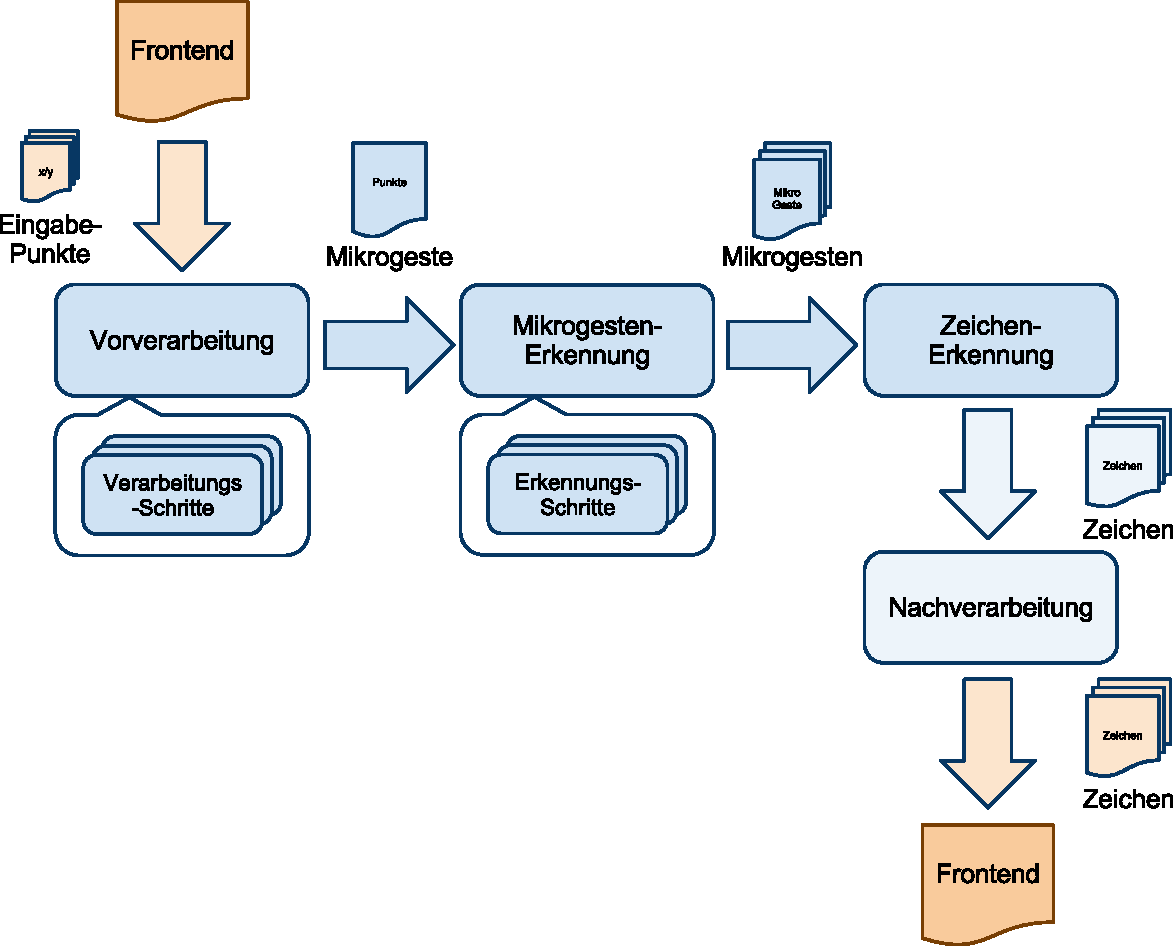
\includegraphics[scale=0.75, bb=10 0 744 460]{img/erkennungs_ablauf.pdf} 
   \caption{Erkennungs-Ablauf}
   \label{fig:erkennungs_ablauf}
\end{figure}

Zuerst soll eine Vorverarbeitung der Eingabe-Punkte durchgeführt werden, in der etwa eine Normierung, eine Glättung, eine Filterung oder ähnliches dieser durchgeführt werden kann. Diese Verarbeitungs-Schritte sollen sich nicht gegenseitig ausschliessen, sollen aber auch optional sein, da einige der dazu möglichen Algorithmen sehr rechenaufwendig sind.

Die zweite Phase soll die Erkennung der Mikrogesten sein. Auf diese soll in mehrere Erkennungs-Schritte aufgeteilt sein, die gegebenenfalls auch deaktiviert werden können.

Als nächstes soll die Zeichen-Erkennung durchgeführt werden. Diese soll allerdings in sich geschlossen funktionieren und nicht zwingend weiter in Teil-Schritte aufgeteilt werden. Das Erkennungs-Verfahren als ganzes soll allerdings austauschbar sein.

Die vierte und letzte Phase soll die Nachverarbeitung der erkannten Zeichen sein. Dies kann etwa bedeuten, das gewisse Zeichen wieder verworfen werden oder das die Gewichtung der Erkennungs-Wahrscheinlichkeit der Zeichen angepasst wird.

\subsubsection{Vorverarbeitung}

\subsubsection{Mikrogesten-Erkennung}

\subsubsection{Zeichen-Erkennung}

\subsubsection{Nachverarbeitung}
%================================================

\section{Design}

(Klassendiagramm, Sequenzdiagramm)
%================================================

\section{Implementation}

(...)
%================================================



	\part{Diskussion}
		\chapter{Ausblick und Erweiterungen}
		\chapter{Schlussfolgerung}


	% Ende Inhalt

	% Glossary
	\glossarystyle{list}
	\makeglossaries

	% Literaturverzeichnis
	\bibliographystyle{plain}
	%\bibliographystyle{geralpha}
	\bibliography{etc/bibliography}{}
	
	% Appendices
	\appendix
	\chapter{Projektplanung}
		% Vorgehen
		\section{SCRUM}
		\section{Sprints}
\end{document}


